\documentclass[a4paper,14pt]{extreport} % формат документа

\usepackage{amsmath}
\usepackage{cmap} % поиск в ПДФ
\usepackage[T2A]{fontenc} % кодировка
\usepackage[utf8]{inputenc} % кодировка исходного текста
\usepackage[english,russian]{babel} % локализация и переносы
\usepackage[left = 2cm, right = 1cm, top = 2cm, bottom = 2 cm]{geometry} % поля
\usepackage{listings}
\usepackage{graphicx} % для вставки рисунков
\usepackage{amsmath}
\usepackage{float}
\usepackage{multirow}
\graphicspath{{pictures/}}
\DeclareGraphicsExtensions{.pdf,.png,.jpg}
\newcommand{\anonsection}[1]{\section*{#1}\addcontentsline{toc}{section}{#1}}

\lstset{ %
	language=python,                % Язык программирования 
	numbers=left,                   % С какой стороны нумеровать          
	frame=single,                    % Добавить рамку
	escapebegin=\begin{russian}\commentfont,
    escapeend=\end{russian},
    literate={Ö}{{\"O}}1
    {Ä}{{\"A}}1
    {Ü}{{\"U}}1
    {ß}{{\ss}}1
    {ü}{{\"u}}1
    {ä}{{\"a}}1
    {ö}{{\"o}}1
    {~}{{\textasciitilde}}1
    {а}{{\selectfont\char224}}1
    {б}{{\selectfont\char225}}1
    {в}{{\selectfont\char226}}1
    {г}{{\selectfont\char227}}1
    {д}{{\selectfont\char228}}1
    {е}{{\selectfont\char229}}1
    {ё}{{\"e}}1
    {ж}{{\selectfont\char230}}1
    {з}{{\selectfont\char231}}1
    {и}{{\selectfont\char232}}1
    {й}{{\selectfont\char233}}1
    {к}{{\selectfont\char234}}1
    {л}{{\selectfont\char235}}1
    {м}{{\selectfont\char236}}1
    {н}{{\selectfont\char237}}1
    {о}{{\selectfont\char238}}1
    {п}{{\selectfont\char239}}1
    {р}{{\selectfont\char240}}1
    {с}{{\selectfont\char241}}1
    {т}{{\selectfont\char242}}1
    {у}{{\selectfont\char243}}1
    {ф}{{\selectfont\char244}}1
    {х}{{\selectfont\char245}}1
    {ц}{{\selectfont\char246}}1
    {ч}{{\selectfont\char247}}1
    {ш}{{\selectfont\char248}}1
    {щ}{{\selectfont\char249}}1
    {ъ}{{\selectfont\char250}}1
    {ы}{{\selectfont\char251}}1
    {ь}{{\selectfont\char252}}1
    {э}{{\selectfont\char253}}1
    {ю}{{\selectfont\char254}}1
    {я}{{\selectfont\char255}}1
    {А}{{\selectfont\char192}}1
    {Б}{{\selectfont\char193}}1
    {В}{{\selectfont\char194}}1
    {Г}{{\selectfont\char195}}1
    {Д}{{\selectfont\char196}}1
    {Е}{{\selectfont\char197}}1
    {Ё}{{\"E}}1
    {Ж}{{\selectfont\char198}}1
    {З}{{\selectfont\char199}}1
    {И}{{\selectfont\char200}}1
    {Й}{{\selectfont\char201}}1
    {К}{{\selectfont\char202}}1
    {Л}{{\selectfont\char203}}1
    {М}{{\selectfont\char204}}1
    {Н}{{\selectfont\char205}}1
    {О}{{\selectfont\char206}}1
    {П}{{\selectfont\char207}}1
    {Р}{{\selectfont\char208}}1
    {С}{{\selectfont\char209}}1
    {Т}{{\selectfont\char210}}1
    {У}{{\selectfont\char211}}1
    {Ф}{{\selectfont\char212}}1
    {Х}{{\selectfont\char213}}1
    {Ц}{{\selectfont\char214}}1
    {Ч}{{\selectfont\char215}}1
    {Ш}{{\selectfont\char216}}1
    {Щ}{{\selectfont\char217}}1
    {Ъ}{{\selectfont\char218}}1
    {Ы}{{\selectfont\char219}}1
    {Ь}{{\selectfont\char220}}1
    {Э}{{\selectfont\char221}}1
    {Ю}{{\selectfont\char222}}1
    {Я}{{\selectfont\char223}}1
    {і}{{\selectfont\char105}}1
    {ї}{{\selectfont\char168}}1
    {є}{{\selectfont\char185}}1
    {ґ}{{\selectfont\char160}}1
    {І}{{\selectfont\char73}}1
    {Ї}{{\selectfont\char136}}1
    {Є}{{\selectfont\char153}}1
    {Ґ}{{\selectfont\char128}}1
}

\begin{document}
\begin{titlepage}

    \begin{table}[H]
        \centering
        \footnotesize
        \begin{tabular}{cc}
            \multirow{8}{*}{
\includegraphics[scale=0.35]{bmstu.jpg}}
            & \\
            & \\
            & \textbf{Министерство науки и высшего образования Российской Федерации} \\
            & \textbf{Федеральное государственное бюджетное образовательное учреждение} \\
            & \textbf{высшего образования} \\
            & \textbf{<<Московский государственный технический} \\
            & \textbf{университет имени Н.Э. Баумана>>} \\
            & \textbf{(МГТУ им. Н.Э. Баумана)} \\
        \end{tabular}
    \end{table}

    \vspace{-2.5cm}

    \begin{flushleft}
        \rule[-1cm]{\textwidth}{3pt}
        \rule{\textwidth}{1pt}
    \end{flushleft}

    \begin{flushleft}
        \small
        ФАКУЛЬТЕТ
        \underline{<<Информатика и системы управления>>\ \ \ \ \ \ \ 
        \ \ \ \ \ \ \ \ \ \ \ \ \ \ \ \ \ \ \ \ \ \ \ \ \ \ \ \ \ \ \ 
    \ \ \ \ \ \ \ \ \ \ \ \ \ \ \ } \\
        КАФЕДРА
        \underline{<<Программное обеспечение ЭВМ и
        информационные технологии>>
        \ \ \ \ \ \ \ \ \ \ \ \ \ \ \ \ \ \ \ \ }
    \end{flushleft}

    \vspace{2cm}

    \begin{center}
        \textbf{Лабораторная работа № 3} \\
        \vspace{0.5cm}
    \end{center}

    \vspace{4cm}

    \begin{flushleft}
        \begin{tabular}{ll}
            \textbf{Дисциплина} & Моделирование.  \\
            \textbf{Тема} & Программно-алгоритмическая реализация моделей на основе  \\
            & ОДУ второго порядка с краевыми условиями II и  III рода. \\
            \\
            \textbf{Студент} & Сиденко А.Г. \\
            \textbf{Группа} & ИУ7-63Б \\
            \textbf{Оценка (баллы)} & \\
            \textbf{Преподаватель} & Градов В.М.   \\
        \end{tabular}
    \end{flushleft}

    \vspace{4cm}

   \begin{center}
        Москва, 2020 г.
    \end{center}

\end{titlepage}

\textbf{Цель работы:} Получение навыков разработки алгоритмов решения краевой задачи при реализации моделей, построенных на ОДУ второго порядка.

\begin{enumerate}
\item Дано:
$$K_0=0.4$$
$$K_N=0.1$$
$$\alpha_0=0.05$$
$$\alpha_N=0.01$$
$$l=10$$
$$T_0=300$$
$$R=0.5$$
$$F_0=50$$

\item Уравнение

\begin{equation}
\frac{d}{dx}\bigg(K(x)\frac{dT}{dx}\bigg)-\frac{2}{R}\alpha(x)T+\frac{2T_0}{R}\alpha(x)=0
\end{equation}

\item Краевые условия

$$
 \begin{cases}
   x=0, ~-k(0)\frac{dT}{dx}=F_0
   \\
   x =l,~-k(l)\frac{dT}{dx}=\alpha_N(T(l)-T_0)
 \end{cases}
$$

Функции $k(x), \alpha(x)$ заданы:

$$k(x)=\frac{a}{x-b}$$, где 

$$a=-K_0b=\frac{K_0K_Nl}{K_0-K_N}, b = \frac{K_Nl}{K_N-K_0}$$

$$\alpha(x)=\frac{c}{x-d}$$, где 

$$c=-\alpha_0d=\frac{\alpha_0\alpha_Nl}{\alpha_0-\alpha_N}, d = \frac{\alpha_Nl}{\alpha_N-\alpha_0}$$

\item Разностная схема

$$
\begin{aligned}
&A_ny_{n-1}-B_ny_n+C_ny_{n+1}=-D_n, 1\le n\le N-1\\
&K_0y_0+M_0y_1=P_0\\
&K_Ny_N+M_Ny_{N-1}=P_N
\end{aligned}
\eqno(2)
$$
, где

$$A_n=\frac{x_{n-\frac{1}{2}}}{h},~B_n=A_n+C_n+p_nh,~C_n=\frac{x_{n+\frac{1}{2}}}{h},~D_n=f_nh$$

Способ вычисления (метод средних):

$$x_{n\pm\frac{1}{2}}=\frac{k_n+k_{n\pm1}}{2}$$

Система совместно с краевыми условиями решается методом прогонки. 

\item Краевые условия

Обозначим:

$$
\begin{aligned}
&F=-k(x)\frac{dT}{dx}\\
&p(x)=\frac{2}{R}\alpha(x)\\
&f(x)=\frac{2T_0}{R}\alpha(x)\\
&p_n=p(x_n), ~f_n=f(x_n)
\end{aligned}
\eqno(3)
$$

Разностные аналоги краевых условий при x=0:

$$y_0\cdot\bigg(x_{\frac{1}{2}} + \frac{h^2}{8}p_{\frac{1}{2}}+\frac{h^2}{4}p_0\bigg)-y_1\cdot\bigg(x_{\frac{1}{2}}-\frac{h^2}{8}p_{\frac{1}{2}}\bigg)=\bigg(hF_0+\frac{h^2}{4}(f_{\frac{1}{2}}+f_0)\bigg)
\eqno(4)
$$

Взято из лекции. 

Можно принять простую аппроксимацию

$$p_{\frac{1}{2}}=\frac{p_0+p_1}{2}$$

$$f_{\frac{1}{2}}=\frac{f_0+f_1}{2}$$

Разностные аналоги краевых условий при x=l, вывод:

Проинтегрируем уравнение 1 с учетом замен 3 на отрезке $[x_{N-\frac{1}{2}},x_N]$

$$-\int^{X_N}_{X_{N-{\frac{1}{2}}}}\frac{dF}{dx}dx-\int^{X_N}_{X_{N-{\frac{1}{2}}}}p(x)Tdx+\int^{X_N}_{X_{N-{\frac{1}{2}}}}f(x)dx=0$$

Второй и третий интегралы вычислим методом трапеций

$$F_{N-\frac{1}{2}}-F_N-\frac{p_{N-\frac{1}{2}}y_{N-\frac{1}{2}}+p_Ny_N}{4}h+\frac{f_{N-\frac{1}{2}}+f_N}{4}h=0$$

Зная

$$F_{N-\frac{1}{2}}=x_{N-\frac{1}{2}}\frac{y_{N-1}-y_N}{h}$$
$$F_N=\alpha_N(y_N-T_0)$$
$$y_{N-\frac{1}{2}}=\frac{y_N+y_{N-1}}{2}$$

\begin{multline*}
\frac{x_{N-\frac{1}{2}}y_{N-1}}{h}-\frac{x_{N-\frac{1}{2}}y_N}{h}-\alpha_Ny_N+\alpha_NT_0-\frac{p_{N-\frac{1}{2}}y_{N-1}}{8}h-\frac{p_{N-\frac{1}{2}}y_N}{8}h-\frac{p_Ny_N}{4}h+\\+\frac{f_{N-\frac{1}{2}}+f_N}{4}h=0
\end{multline*}

\begin{multline*}
y_N\cdot\bigg(-\frac{x_{N-\frac{1}{2}}}{h}-\alpha_N-\frac{p_N}{4}h-\frac{p_{N-\frac{1}{2}}}{8}h\bigg) + y_{N-1}\cdot\bigg (\frac{x_{N-\frac{1}{2}}}{h}-\frac{p_{N-\frac{1}{2}}}{8}h\bigg) =\\
=-\bigg(\alpha_NT_0+\frac{f_{N-\frac{1}{2}}+f_N}{4}h\bigg)~~~~(5)
\end{multline*}

Соответственно из этих краевых условий (формулы 4, 5) находим коэффициенты для системы 2: $K_0,~K_N,~M_0,~M_N,~P_0,~P_N$. 

\item Метод прогонки

Для решения системы 2 используется метод прогонки. 

Метод состоит из двух этапов прямой ход и обратный ход (прогоночные коэффициенты и нахождение неизвестных). 

1 этап:

По формуле 6 вычисляются начальные значения прогоночных коэффициентов $\varepsilon_1, \eta_1$. 

$$
\begin{aligned}
&\varepsilon_1=-\frac{M_0}{K_0}\\
&\eta_1=\frac{P_0}{K_0}
\end{aligned}
\eqno(6)
$$

По формуле 7 вычисляются массивы прогоночных коэффициентов $\varepsilon, \eta$. 

$$y_n=\underbrace{\frac{C_n}{B_n-A_n\varepsilon_n}}_{\varepsilon_{n+1}}y_{n+1}+\underbrace{\frac{D_n+A_n\eta_n}{B_n-A_n\varepsilon_n}}_{\eta_{n+1}}\eqno(7)$$

2 этап:

По формуле 8 определяется $y_N$ значение функции в последней точке. 

$$y_N=\frac{P_N-M_N\eta_N}{K_N+M_N\varepsilon_N} \eqno(8)$$

И по основной прогоночной формуле 9 находятся все значения неизвестных $y_n$. 

$$y_n=\varepsilon_{n+1}y_{n+1}+\eta_{n+1}\eqno(9)$$


Таким образом, массив, полученный после прогонки и есть искомый массив T(x). 

\end{enumerate}

\textbf{Приведем листинг. }

\begin{lstlisting}[caption=Заданные параметры]
K0 = 0.4
KN = 0.1
alpha0 = 0.05
alphaN = 0.01
l = 10
T0 = 300
R = 0.5
F0 = 50
h = 0.1
\end{lstlisting}

\begin{lstlisting}[caption=Параметры коэффициентов теплопроводности материала стержня и теплоотдачи при обдуве]
b = (KN * l) / (KN - K0)
a = - K0 * b
d = (alphaN * l) / (alphaN - alpha0)
c = - alpha0 * d
\end{lstlisting}

\begin{lstlisting}[caption=Коэффициенты теплопроводности материала стержня и теплоотдачи при обдуве]
def k(x):
    return a / (x - b)

def alpha(x):
    return c / (x - d)
\end{lstlisting}

\begin{lstlisting}[caption=Выполненные замены]
def p(x):
    return 2 * alpha(x) / R

def f(x):
    return 2 * alpha(x) * T0 / R
\end{lstlisting}

\begin{lstlisting}[caption=Метод средних для вычисления значения Х]
def x_plus_1_2(x):
    return (k(x) + k(x + h)) / 2

def x_minus_1_2(x):
    return (k(x) + k(x - h)) / 2
\end{lstlisting}

\begin{lstlisting}[caption=Параметры разностной схемы]
def A(x):
    return x_minus_1_2(x) / h

def C(x):
    return x_plus_1_2(x) / h

def B(x):
    return A(x) + C(x) + p(x) * h

def D(x):
    return f(x) * h
\end{lstlisting}

\begin{lstlisting}[caption=Краевые условия]
K0 = x_plus_1_2(0) + h*h*(p(0) + p(h)) / 16 + h*h*p(0) / 4
M0 = -(x_plus_1_2(0) - h * h * (p(0) + p(h)) / 16)
P0 = h * F0 + h * h / 4 * ((f(0) + f(h)) / 2 + f(0))

KN = -x_minus_1_2(l)/h- alphaN- p(l)*h/4 - (p(l)+p(l-h))*h/16
MN = x_minus_1_2(l) / h - (p(l) + p(l - h)) * h / 16
PN = -(alphaN * T0 + ((f(l) + f(l - h)) / 2 + f(l)) * h / 4)
\end{lstlisting}

\begin{lstlisting}[caption=Метод прогонки]
def run_through():
    # Прямой ход
    eps = [0, -M0 / K0]
    eta = [0, P0 / K0]

    x = h
    n = 1
    while (x + h < l):
        eps.append(C(x) / (B(x) - A(x) * eps[n]))
        eta.append((D(x) + A(x) * eta[n])/(B(x)-A(x) * eps[n]))
        n += 1
        x += h

    # Обратный ход
    t = [0] * (n + 1)
    t[n] = (PN - MN * eta[n]) / (KN + MN * eps[n])

    for i in range(n - 1, -1, -1):
        t[i] = eps[i + 1] * t[i + 1] + eta[i + 1]

    return t
\end{lstlisting}

\newpage 
\textbf{Результаты работы программы. }

\begin{enumerate}
\item График зависимости температуры от координаты при заданных выше параметрах.

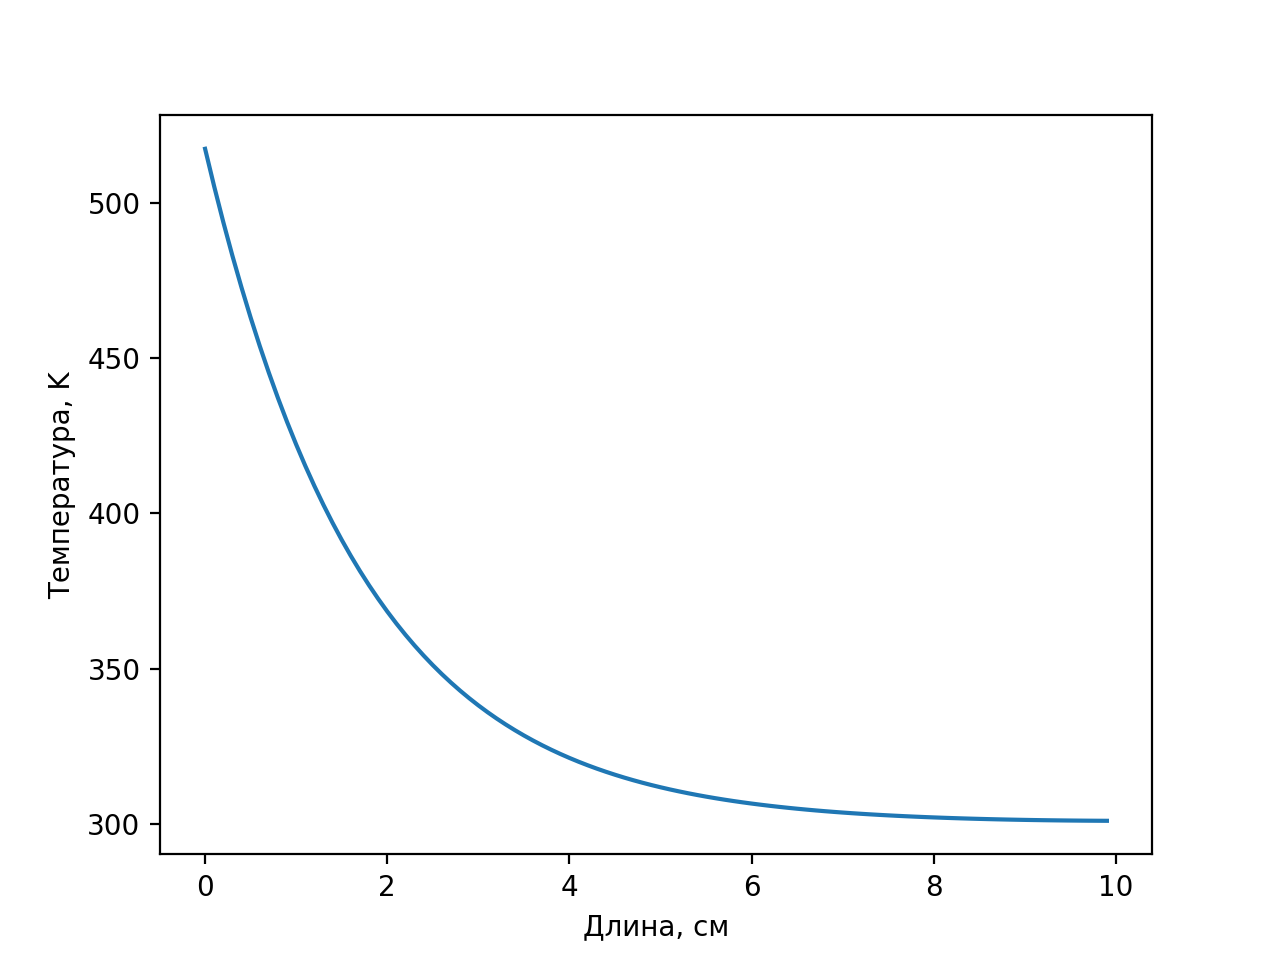
\includegraphics[scale=0.9]{graph1}
\item График зависимости при $F_0$ = -10. 

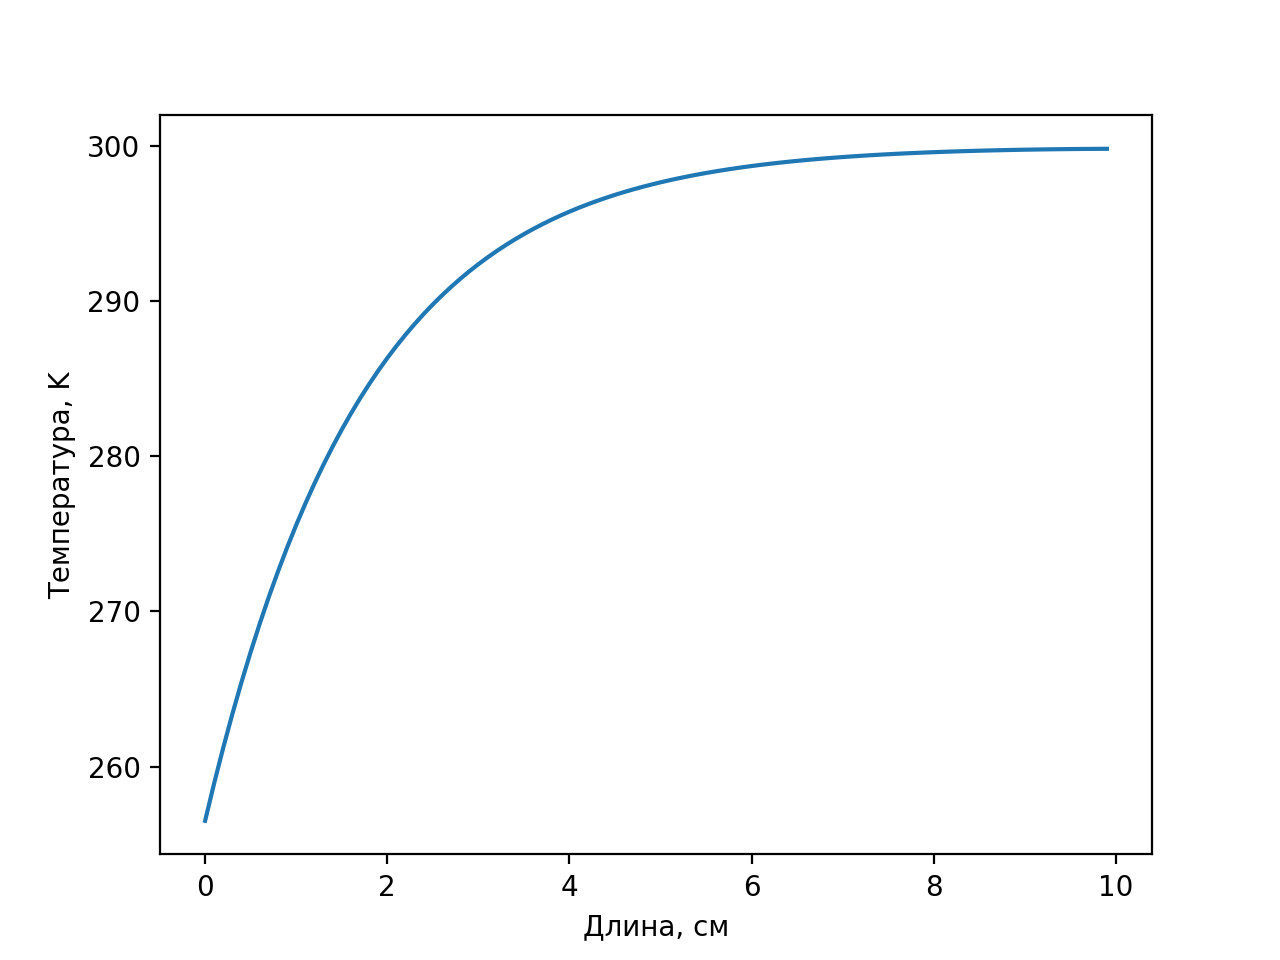
\includegraphics[scale=0.9]{graph2}
\item График зависимости при увеличенных значениях $\alpha$ (например, в 3 раза). 

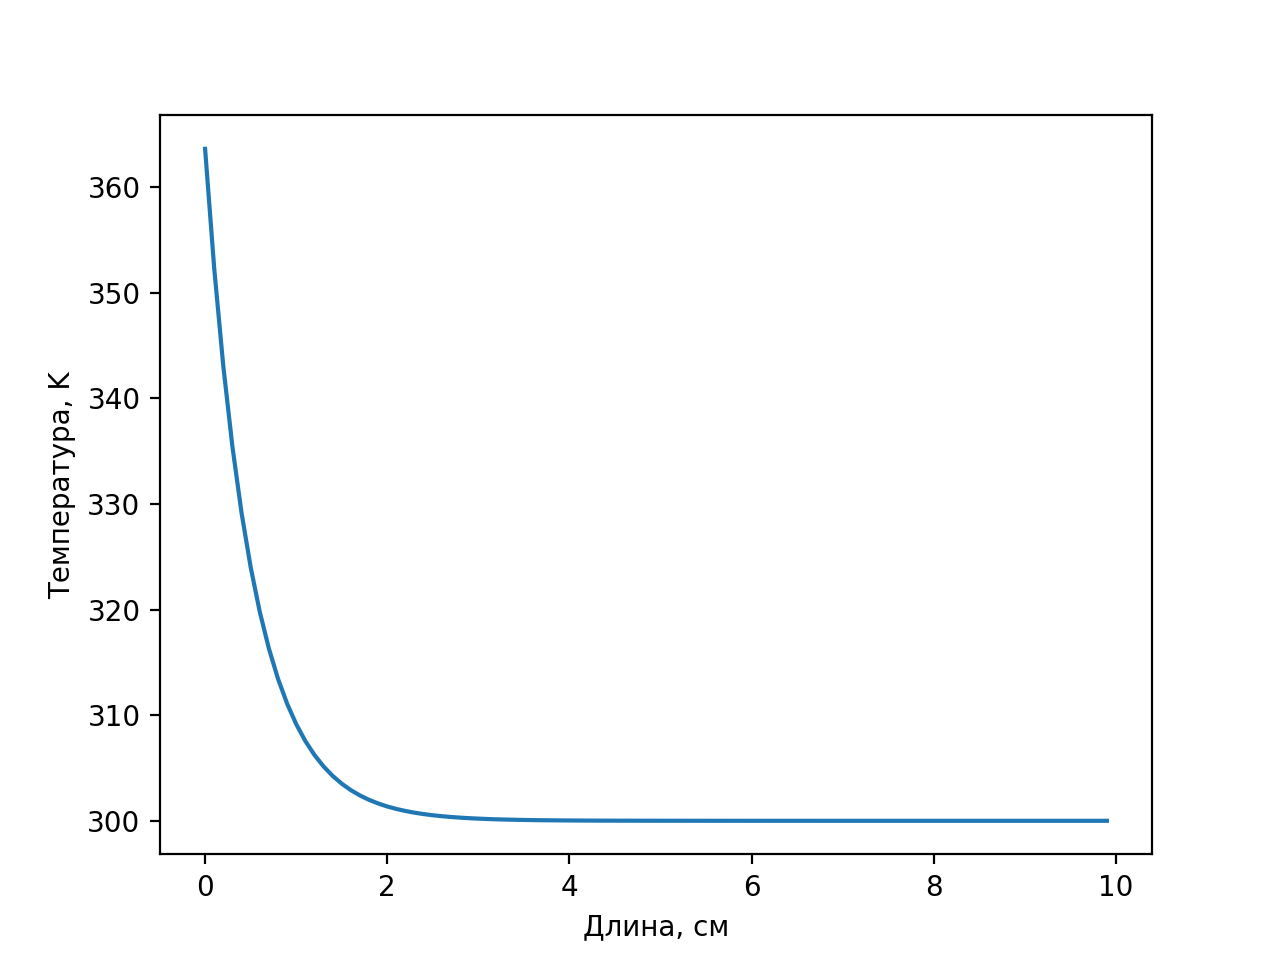
\includegraphics[scale=0.9]{graph3}
\item График зависимости при $F_0$ = 0. 

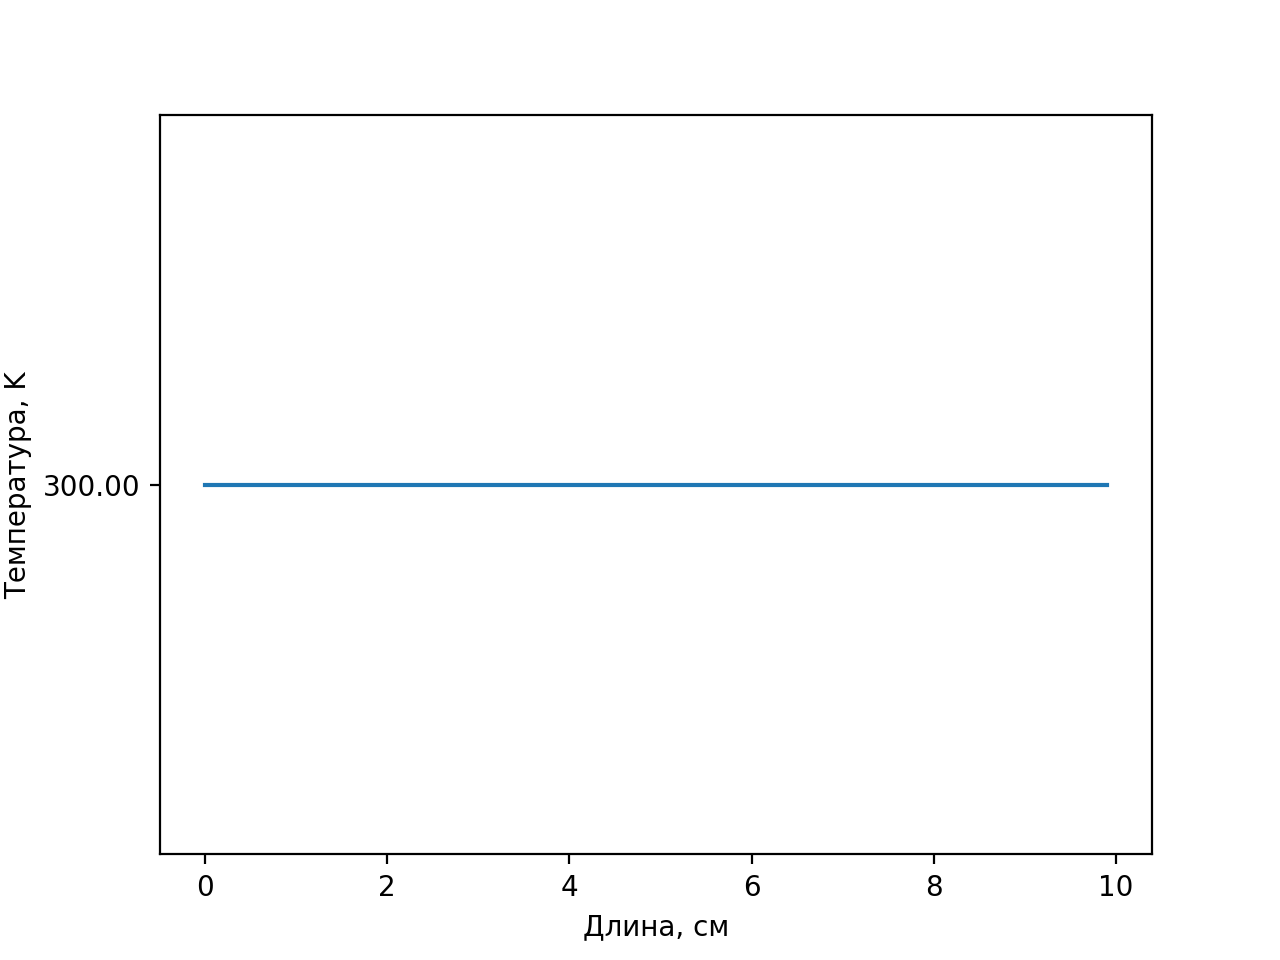
\includegraphics[scale=0.9]{graph4}
\end{enumerate}

\newpage
\textbf{Ответы на вопросы. }

\begin{enumerate}
\item Какие способы тестирования программы можно предложить?

3 способа тестирования: 
\begin{enumerate}
\item Задаем тепловой поток отрицательным, это означает что идет съем тепла с левого торца $x=0$, а значит температура от 0 до $l$ будет увеличиваться. (производная положительная)
\item Увеличиваем коэффициент теплоотдачи (стержень при том же самом тепловом потоке отдает больше тепла). А следовательно температура снижается, а скорость снижения температуры (от длины стержня) увеличивается. 
\item Тепловой поток устанавливаем в 0. Съема тепла не происходит, причин для нагрева нет. А значит стержень так и останется при температуре окружающей среды. 
\end{enumerate}

\item Получите  простейший разностный аналог нелинейного краевого условия при  $x=l$, $$-k(l)\frac{dT}{dx}=\alpha_N(T(l)-T_0)+\varphi(T)$$,
где $\varphi(T)$ заданная функция.

Производную аппроксимируйте односторонней разностью.

Построим простейшую разностную схему методом разностной апроксимации на равномерной сетке с шагом h. 

Тогда в любой точке разностный аналог:

$$\frac{dT}{dx}=\frac{T(x+h)-T(x)}{h}$$

Тогда при $x=l$:

$$\frac{dT}{dx}=\frac{T_{l+1}-T_l}{h}$$

И тогда

$$-k_l\frac{T_{l}-T_{l-1}}{h}=\alpha_N(T_l-T_0)+\varphi(T_l)$$, где $T_l=T(l), k_l=k(l)$

$$-k_lT_{l}+k_lT_{l-1}=\alpha_NhT_l-\alpha_NhT_0+\varphi(T_l)h$$

$$-(k_l+\alpha_Nh)T_{l}+k_lT_{l-1}=\varphi(T_l)h-\alpha_NhT_0$$

\item Опишите алгоритм применения метода прогонки, если при $x=0$ краевое условие линейное (как в настоящей работе), а при $x=l$, как в п.2.

$$
 \begin{cases}
   x=0, ~-k(0)\frac{dT}{dx}=F_0
   \\
   x =l,~-k(l)\frac{dT}{dx}=\alpha_N(T(l)-T_0) + \varphi(T)
 \end{cases}
$$

Изменим направление прогонки, т.е. прогоночные коэффициенты определять справа налево, а функцию - слева направо. Такая прогонка называется левой. В этом случае основная прогоночная формула записывается в виде

$$y_n=\varepsilon_{n-1}y_{n-1}+\eta_{n-1}$$

Принимая простейшую (первого порядка точности) аппроксимацию краевого условия при $x=0$, получим его разностный аналог

$$-k_0\frac{T_1-T_0}{h}=F_0$$

$$-k_0T_1+k_0T_0=F_0h$$

$$
 \begin{cases}
   \varepsilon_0=1
   \\
   \eta_0=-\frac{F_0h}{k_0}
 \end{cases}
$$

Аналогичная разностная аппроксимация правого краевого условия имеет вид:

$$-(k_l+\alpha_Nh)T_{l}+k_lT_{l-1}=\varphi(T_l)h-\alpha_NhT_0$$

$$-(k_l+\alpha_Nh)T_{l}+k_l\frac{T_{l}-\eta_{l-1}}{\varepsilon_{l-1}}=\varphi(T_l)h-\alpha_NhT_0$$

Откуда получаем уравнение для определения $T_0$. 

$$\varphi(T_l)h-(k_l+\alpha_Nh-\frac{k_l}{\varepsilon_{l-1}})T_l=\frac{k_l\eta_{l-1}}{\varepsilon_{l-1}}-\alpha_NhT_0$$

\item Опишите алгоритм определения единственного значения сеточной функции $y_p$ в одной заданной точке $p$. Использовать встречную прогонку, т.е. комбинацию правой и левой (лекция №8). Краевые условия линейные.

Комбинируя левую и правую прогонки, получаем метод встречных прогонок. 

Пусть $i=p$, где $0<p<N$. 

Тогда в области $0\le i \le p+1$ прогоночные коэффициенты $\alpha_i, \beta_i$ (правая прогонка):

$$\alpha_{i+1}=\frac{C_i}{B_i-\alpha_iA_i}$$

$$\beta_{i+1}=\frac{A_i\beta_i+D_i}{C_i-\alpha_iA_i}$$

А в области $p\le i \le N$ прогоночные коэффициенты $\varepsilon_i, \eta_i$ (левая прогонка):

$$\varepsilon_{i}=\frac{C_i}{B_i-\varepsilon_{i+1}A_i}$$

$$\eta_{i}=\frac{A_i\eta_{i+1}+D_i}{B_i-\varepsilon_{i+1}A_i}$$

Тогда при $i=p$:

$$y_p=\alpha_{p+1}y_{p+1}+\beta_{p+1},~~y_{p+1}=\varepsilon_{p+1}y_{p}+\eta_{p+1}$$

И тогда:

$$y_{p}=\frac{\beta_{p+1}+\alpha_{p+1}\eta_{p+1}}{1-\alpha_{p+1}\varepsilon_{p+1}}$$

\end{enumerate}

\end{document}